\documentclass[tikz,border=10pt]{standalone}
\usepackage{pgfplots}
\usepackage{xcolor}
\definecolor{arr2flatcolour}{RGB}{82,139,189}
\definecolor{minnesotacolour}{RGB}{230,171,2}
\definecolor{gaussiancolour}{RGB}{0,114,189}
\definecolor{rhscolour}{RGB}{180,41,104}
\definecolor{arr2minncolour}{RGB}{230,41,189}
\definecolor{arr2bumpcolour}{RGB}{82,189,189}
\pgfplotsset{compat=1.18}

\begin{document}
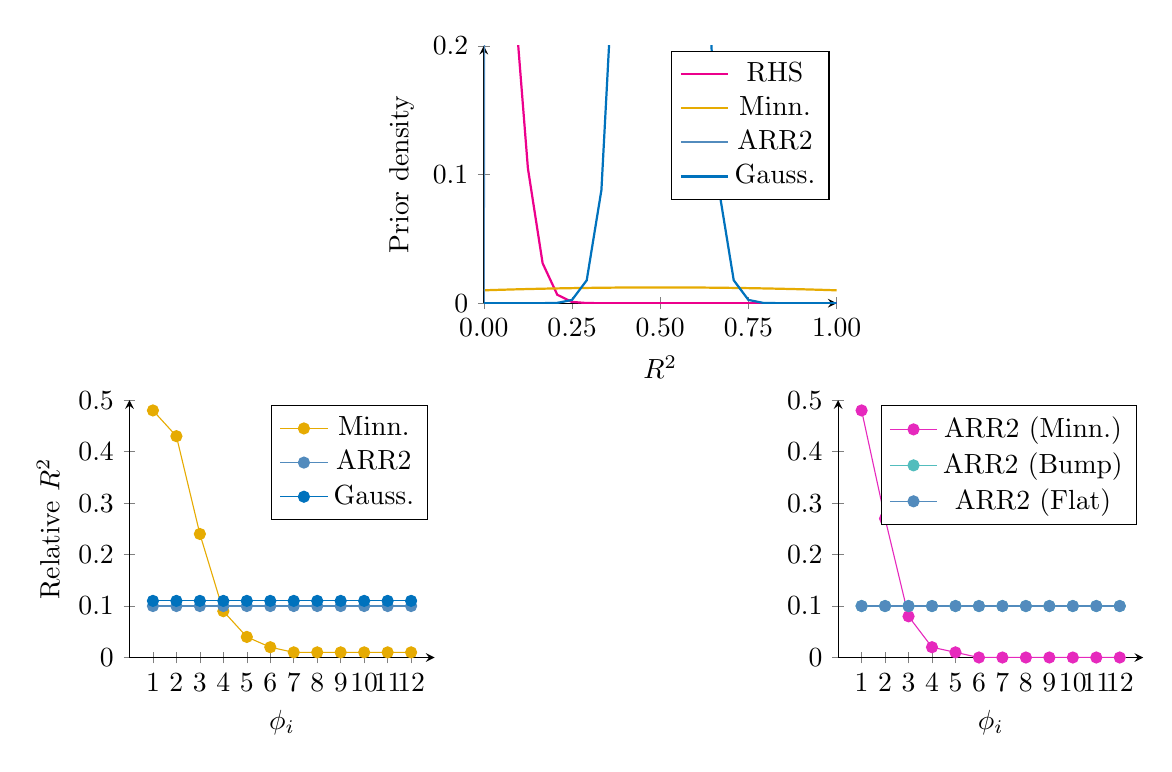
\begin{tikzpicture}
\begin{scope}[shift={(0,0)}]
\begin{axis}[
    axis lines=left,
    xlabel = {\(R^2\)},
    ylabel = {Prior density},
    ymin=0, ymax=0.2,
    xtick={0,0.25,0.5,0.75,1},
    xticklabels={0.00,0.25,0.50,0.75,1.00},
    ytick={0,0.1,0.2},
    width=0.5\textwidth,
    height=0.4\textwidth
]
\addplot [color=magenta, thick, domain=0:1] {0.5*exp(-100*(x-0)^2)};
\addlegendentry{RHS}
\addplot [color=minnesotacolour, thick, domain=0:1] {0.9*pow(0.1,2)*x*(1-x)+0.01};
\addlegendentry{Minn.}
\addplot [color=arr2flatcolour, thick, domain=0:1] {0.6*x^-0.9*(1-x)^-0.9};
\addlegendentry{ARR2}
\addplot [color=gaussiancolour, thick, domain=0:1] {3*pow(x*(1-x),0.5)*exp(-100*pow(x-0.5,2))};
\addlegendentry{Gauss.}
\end{axis}
\end{scope}

\begin{scope}[shift={(-4.5,-4.5)}]
\begin{axis}[
    axis lines=left,
    ylabel = {Relative $R^2$},
    xlabel = {\(\phi_i\)},
    xmin=0, xmax=13,
    xtick={1,2,...,12},
    ytick={0,0.1,0.2,0.3,0.4,0.5},
    width=0.45\textwidth,
    height=0.4\textwidth,
    ymin=0, ymax=0.5
]
\addplot [color=minnesotacolour, mark=*, mark size=2pt] coordinates {(1,0.48) (2,0.43) (3,0.24) (4,0.09) (5,0.04) (6,0.02) (7,0.01) (8,0.01) (9,0.01) (10,0.01) (11,0.01) (12,0.01)};
\addlegendentry{Minn.}
\addplot [color=arr2flatcolour, mark=*, mark size=2pt] coordinates {(1,0.1) (2,0.1) (3,0.1) (4,0.1) (5,0.1) (6,0.1) (7,0.1) (8,0.1) (9,0.1) (10,0.1) (11,0.1) (12,0.1)};
\addlegendentry{ARR2}
\addplot [color=gaussiancolour, mark=*, mark size=2pt] coordinates {(1,0.11) (2,0.11) (3,0.11) (4,0.11) (5,0.11) (6,0.11) (7,0.11) (8,0.11) (9,0.11) (10,0.11) (11,0.11) (12,0.11)};
\addlegendentry{Gauss.}
\end{axis}
\end{scope}

\begin{scope}[shift={(4.5,-4.5)}]
\begin{axis}[
    axis lines=left,
    ylabel = {},
    xlabel = {\(\phi_i\)},
    xmin=0, xmax=13,
    xtick={1,2,...,12},
    ytick={0,0.1,0.2,0.3,0.4,0.5},
    width=0.45\textwidth,
    height=0.4\textwidth,
    ymin=0, ymax=0.5
]
\addplot [color=arr2minncolour, mark=*, mark size=2pt] coordinates {(1,0.48) (2,0.27) (3,0.08) (4,0.02) (5,0.01) (6,0) (7,0) (8,0) (9,0) (10,0) (11,0) (12,0)};
\addlegendentry{ARR2 (Minn.)}
\addplot [color=arr2bumpcolour, mark=*, mark size=2pt] coordinates {(1,0.1) (2,0.1) (3,0.1) (4,0.1) (5,0.1) (6,0.1) (7,0.1) (8,0.1) (9,0.1) (10,0.1) (11,0.1) (12,0.1)};
\addlegendentry{ARR2 (Bump)}
\addplot [color=arr2flatcolour, mark=*, mark size=2pt] coordinates {(1,0.1) (2,0.1) (3,0.1) (4,0.1) (5,0.1) (6,0.1) (7,0.1) (8,0.1) (9,0.1) (10,0.1) (11,0.1) (12,0.1)};
\addlegendentry{ARR2 (Flat)}
\end{axis}
\end{scope}
\end{tikzpicture}
\end{document}